\documentclass[tikz, border=5mm]{standalone}
\usepackage{textcomp}
\usetikzlibrary{arrows.meta,decorations.markings,fit,calc, positioning}

\definecolor{componentColor}{RGB}{210,210,210}
\definecolor{systemColor}{RGB}{230,230,230}
\usepackage{amsmath}
\usepackage{amsfonts}
\usepackage{amssymb}
\tikzset{component/.append style={fill=componentColor, align=center, draw, minimum width=3.5cm, minimum height=1.5cm, rounded corners=.3cm, font=\large}}
\tikzset{system/.style={component, fill=systemColor, rounded corners=0cm}}
\tikzset{interface/.style={system, fill=systemColor, minimum size=1.6cm}}

\begin{document}

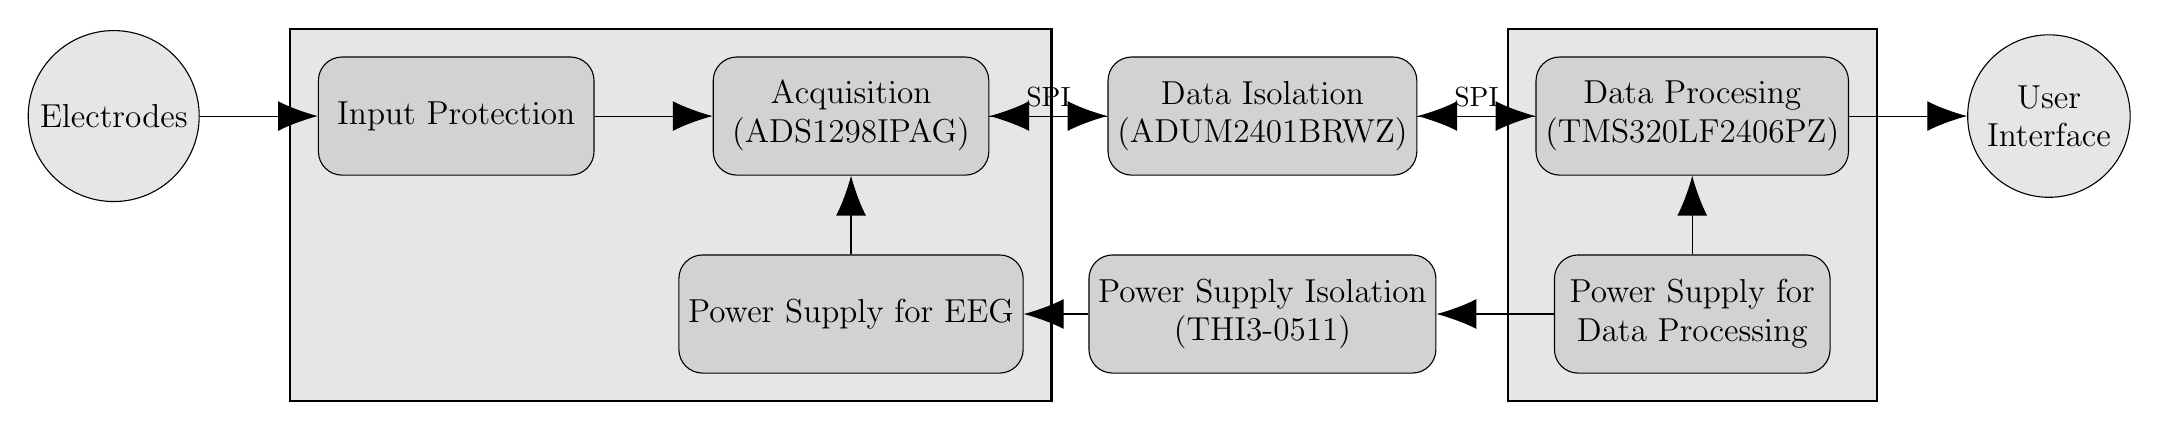
\begin{tikzpicture}[node distance=1cm and 1.5cm]
% Nodes
\pgfdeclarelayer{background}) 
\pgfsetlayers{background,main}

\node (Electrodes) [circle, interface] {Electrodes};
\node (InputProtection) [component, right=of Electrodes] {Input Protection};
\node (Acquisition) [component, right=of InputProtection] {Acquisition\\ (ADS1298IPAG)};
\node (EEGPowerSupply) [component, below=of Acquisition] {Power Supply for EEG};

\node (DataIsolation) [component, right=of Acquisition] {Data Isolation \\ (ADUM2401BRWZ)};
\node (PowerSupplyIsolation) [component, below=of DataIsolation] {Power Supply Isolation \\ (THI3-0511)};

\node (DataProcesing) [component, right=of DataIsolation] {Data Procesing\\ (TMS320LF2406PZ)};
\node (DataProcessingPowerSupply) [component, below=of DataProcesing] {Power Supply for\\ Data Processing};
\node (UserInterface) [circle, interface, right=of DataProcesing] {User\\ Interface};


\begin{pgfonlayer}{background}
\node[system, draw, thick, inner xsep=1em, inner ysep=1em, fit= (InputProtection) (Acquisition) (EEGPowerSupply) ] {};
\end{pgfonlayer}

\begin{pgfonlayer}{background}
\node[system, draw, thick, inner xsep=1em, inner ysep=1em, fit= (DataProcesing) (DataProcessingPowerSupply) ] {};
\end{pgfonlayer}

% Connectors
\begin{scope}[->]

\draw [-{Latex[scale=3.0]}] (Electrodes) -- node[anchor=west, minimum width=.25cm, draw=none] {} (InputProtection);
\draw [-{Latex[scale=3.0]}] (InputProtection) -- node[anchor=west, minimum width=.25cm, draw=none] {} (Acquisition);

\draw [-{Latex[scale=3.0]}] (Acquisition) -- node[anchor=south, minimum width=.25cm, draw=none] {SPI} (DataIsolation);
\draw [-{Latex[scale=3.0]}] (DataIsolation) -- node[anchor=west, minimum width=.25cm, draw=none] {} (Acquisition);


\draw [-{Latex[scale=3.0]}] (DataProcesing) -- node[anchor=south, minimum width=.25cm, draw=none] {SPI} (DataIsolation);
\draw [-{Latex[scale=3.0]}] (DataIsolation) -- node[anchor=west, minimum width=.25cm, draw=none] {} (DataProcesing);


\draw [-{Latex[scale=3.0]}] (DataProcesing) -- node[anchor=west, minimum width=.25cm, draw=none] {} (UserInterface);

 
\draw [-{Latex[scale=3.0]}] (EEGPowerSupply) -- node[anchor=west, minimum width=.25cm, draw=none] {} (Acquisition);
\draw [-{Latex[scale=3.0]}] (DataProcessingPowerSupply) -- node[anchor=west, minimum width=.25cm, draw=none] {} (DataProcesing);


\draw [-{Latex[scale=3.0]}] (DataProcessingPowerSupply) -- node[anchor=south, minimum width=.25cm, draw=none] {} (PowerSupplyIsolation);
\draw [-{Latex[scale=3.0]}] (PowerSupplyIsolation) -- node[anchor=west, minimum width=.25cm, draw=none] {} (EEGPowerSupply);




\end{scope}



\end{tikzpicture}
\end{document}
